\documentclass[../../Problems]{subfiles}
\begin{document}
\subsection{Gray Code}
A gray code is a rearrangement of binary numbers such that any 2 consecutive numbers differ only in 1 bit.

A simple way to generate n-bit gray code is given below
\begin{itemize}	
	\item Start with an array of $2$ numbers $A = \{0, 1\}$
	\item Repeat the below steps $n-1$ times
	\begin{itemize}
		\item Reverse the array $A$ to get array $A^\prime$  and then append $A^\prime$  to $A$.
		\item Append $0$ to the left of the first half elements of $A$ and\\
		Append $1$ to the left of the second half elements of $A$.
	\end{itemize}
\end{itemize}
\begin{figure}[H]
	\centering
	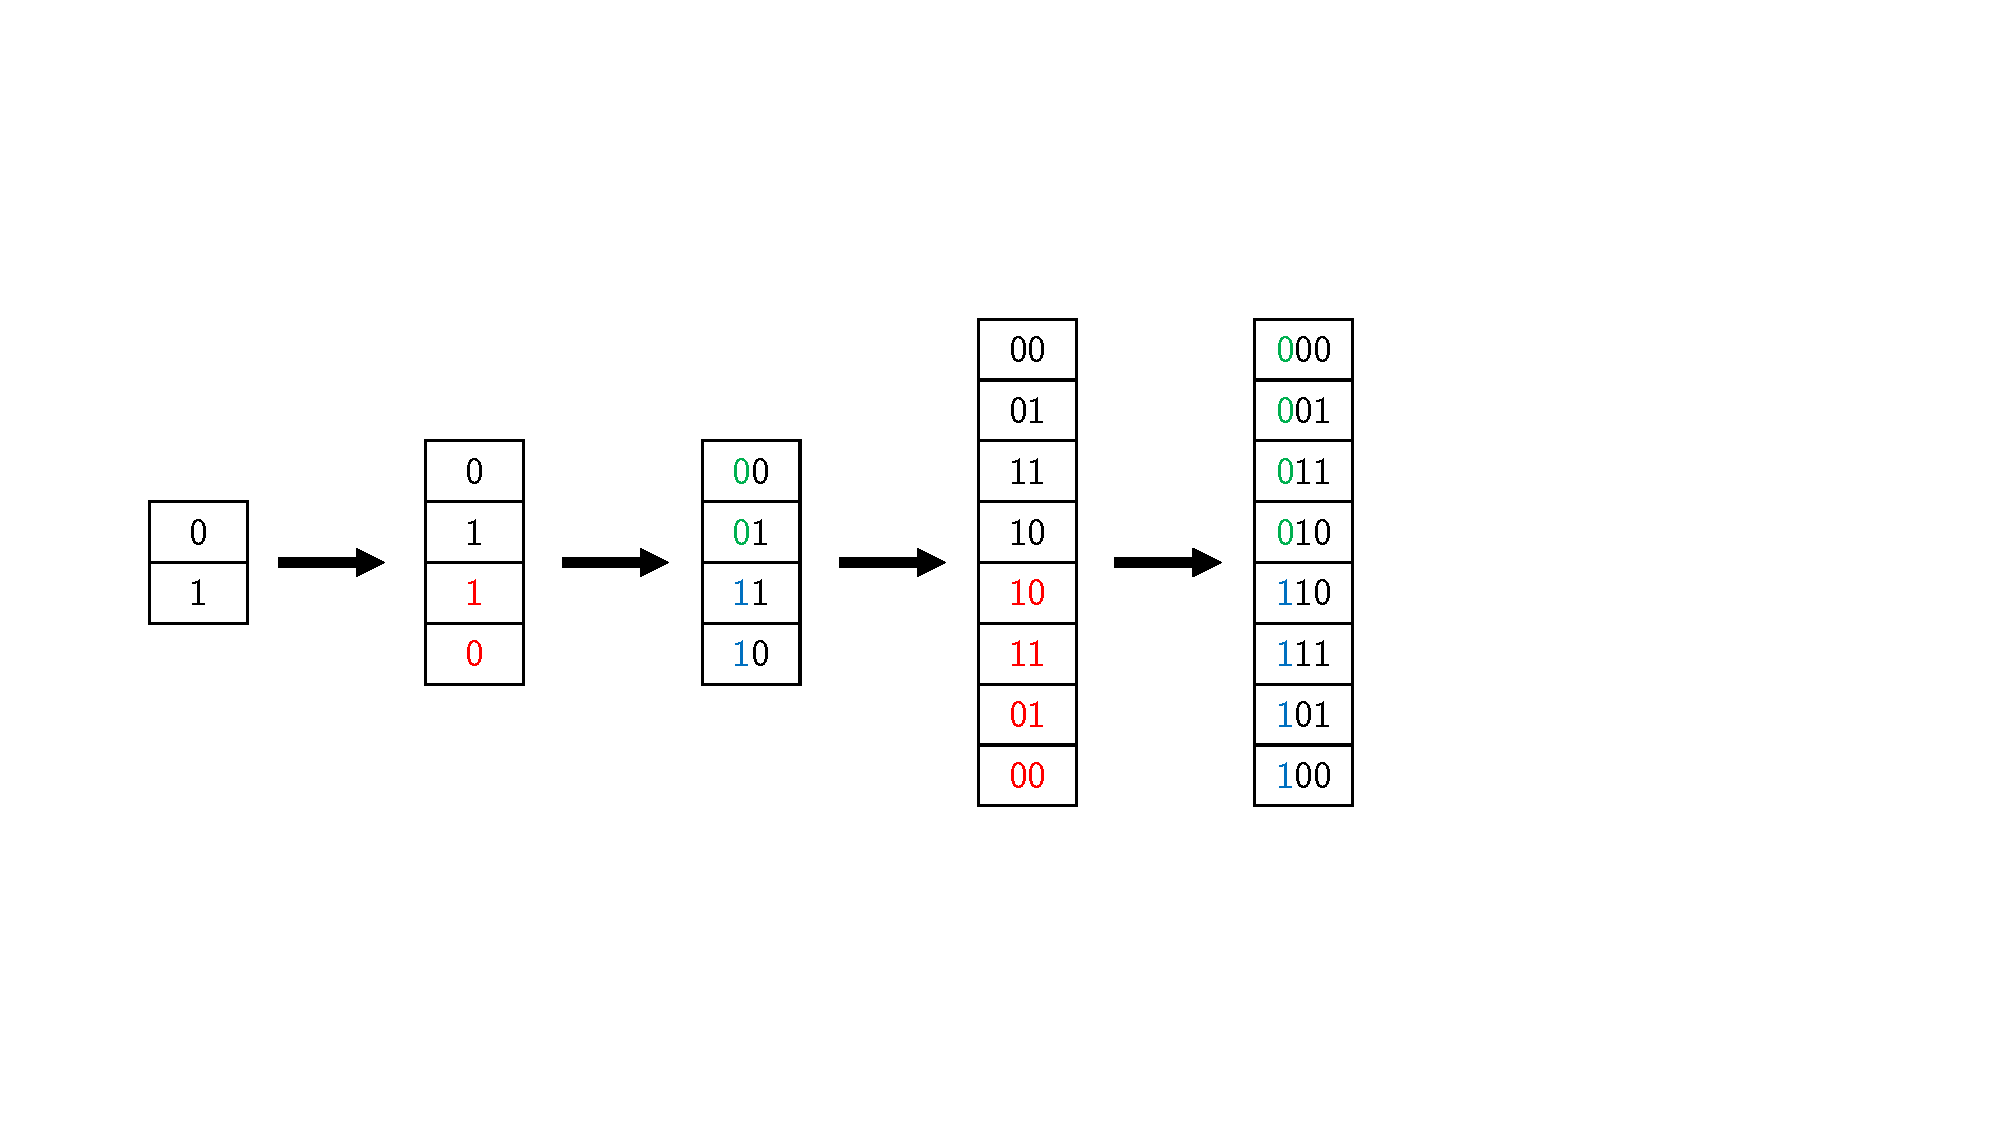
\includegraphics[width = 0.7\linewidth]{Gray Code.pdf}
	\caption{Gray Code -- Generation}
\end{figure}
\vspace{-2em}
\textbf{Problem Statement:}\\
For a given $n$, generate its corresponding Gray Code (i.e. first $2^n$ elements).
\begin{testcasesMore}
	{$n$\hfill(integer)}
	{$2^n$ numbers denoting Gray Code}
	{$1 \leq n \leq 10$}
	{3}
	{000\\001\\011\\010\\110\\111\\101\\100}
	{https://github.com/paramrathour/CS-101/tree/main/Test Cases/Gray Code/Input.txt}
	{https://github.com/paramrathour/CS-101/tree/main/Test Cases/Gray Code/Output.txt}
	{https://github.com/paramrathour/CS-101/tree/main/Starter Codes/Gray Code.cpp}
\end{testcasesMore}
\begin{funvideo}
\href{https://youtu.be/To7Ll5AGboI}{Maths Behind How Wireless Communication Works $\mid$ Quadrature Phase Shift Keying -- Stand-up Maths}
\end{funvideo}
\end{document}